\documentclass[tikz,border=4pt]{standalone}
\usepackage{amsmath}
\definecolor{curveblue}{HTML}{245C86}
\begin{document}
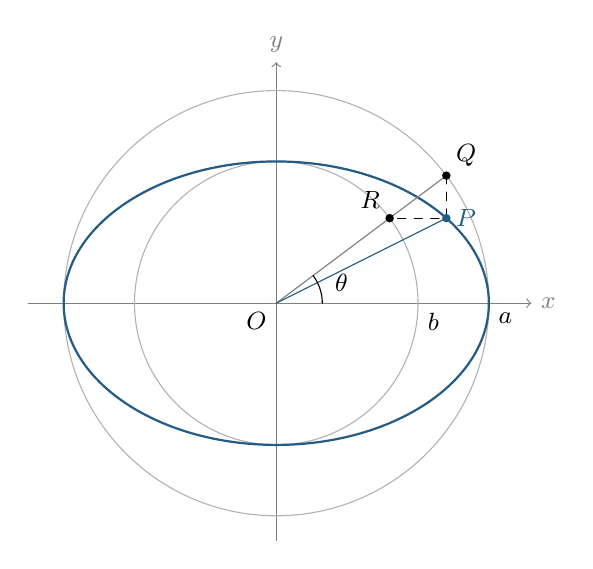
\begin{tikzpicture}[font=\small,line cap=round,scale=.9]
\draw[gray,->](-3.5,0)--(3.6,0)node[right]{$x$};
\draw[gray,->](0,-3.35)--(0,3.4)node[above]{$y$};
\draw[gray!60](0,0)circle(3) (0,0)circle(2);
\draw[curveblue,thick](0,0)ellipse[x radius=3,y radius=2];
\draw[gray](0,0)--(2.4,1.8);
\draw[dashed](2.4,1.8)--(2.4,1.2)--(1.6,1.2);
\draw[curveblue](0,0)--(2.4,1.2);
\draw(.65,0)arc[start angle=0,end angle=36.8699,radius=.65];
\node at(.92,.29){$\theta$};
\fill(2.4,1.8)circle(1.7pt)node[above right]{$Q$};
\fill(1.6,1.2)circle(1.7pt)node[above left]{$R$};
\fill[curveblue](2.4,1.2)circle(1.7pt)node[right]{$P$};
\node[below left]at(0,0){$O$};
\node[below right]at(3,0){$a$};\node[below right]at(2,0){$b$};
\end{tikzpicture}
\end{document}
